\documentclass[11pt]{article}
\usepackage[T1]{fontenc}
\usepackage[margin=0.82in]{geometry}
\usepackage{amsmath,booktabs,microtype}
\usepackage{pgfplots}
\pgfplotsset{compat=1.18}
\usepackage[colorlinks=true,urlcolor=blue,citecolor=blue,linkcolor=blue]{hyperref}
\setlength{\emergencystretch}{2em}
\title{When Does Personalization Earn the Route?\\A Full-Catalog Temporal Study of Guarded Recommendation}
\author{Ahnaf An Nafee}
\date{24 September 2026}

\begin{document}
\maketitle

\begin{abstract}
An offline recommender may look accurate when it reorders familiar items yet fail to recover a later choice from the full catalog. We ask when a personalized challenger has enough evidence to replace a popularity route. Using global temporal splits of Amazon Reviews'23, we train on earlier reviews, retain test targets absent from the training catalog as misses, and fix the decision before opening the Musical Instruments test split. On 35,905 eligible requests, the selected co-review hybrid scores 0.008681 NDCG@10 against 0.008007 for recent popularity, a paired difference of 0.000674 (user-cluster bootstrap 95\% interval [0.000040, 0.001338]). A subsequent two-tower model improves on popularity but not on the active hybrid, so it remains in shadow. We also test what the hybrid leaves unread. Ratings and review age yield positive differences on the validation cohort, but their configurations were selected there and require fresh evaluation. A phrase-to-products arm answers a stated sentence; reconstructed prior-review wording fails to improve the frozen ranking on either full test split. Target-linked external queries show greater reach, but do not represent requests observed from these reviewers. The accompanying service exposes active and shadow rankings with explicit fallbacks. Our result is a bounded comparison and an inspectable routing decision, not evidence of online impact.
\end{abstract}

\noindent\textbf{Keywords:} recommender systems; full-catalog evaluation; temporal split; model selection; neural retrieval; fallback routing; already-held evidence; preference elicitation; phrase-to-products retrieval

\section{Introduction}
A recommender can predict a reviewer's rating of a known product yet fail when asked to find that product among thousands of candidates. Retrieval has to contend with an incomplete training catalog, a changing population, and products the user has never encountered. It also has to choose what to serve when a personalized model offers only a marginal offline improvement. Global time boundaries matter to this choice because future interactions can otherwise enter training or model selection~\cite{ji2023leakage,gusak2025time}.

We study a concrete serving decision: when has a personalized challenger earned the route from a popularity baseline? The baseline is itself selected on validation from lifetime and recent popularity. Against it we test a train-only co-review hybrid, fixing its blend weight and a paired uncertainty gate before opening the next category's test split. We then ask whether a compact two-tower retriever should displace that active hybrid. These models use established methods; the object of study is the decision made with them under a visible candidate set, time boundary, and fallback rule.

The fixed hybrid produces a small positive difference on Musical Instruments, a previously unopened category in the same benchmark. That result supports a bounded claim about this protocol, while the later neural challenger illustrates why improvement over popularity is insufficient if a stronger route is already active. It also leaves a practical question: which signals does the selected route ignore? Its scorer reads the last twenty reviewed products without their ratings or review times, although those fields and older history remain in the archive. We examine whether rereading them changes the ranking, what a hindsight-oracle interview adds, and whether a separate phrase-to-products route can answer a stated request. Each extension is compared with the selected route, with its evidential status made explicit; adding a capability alone does not justify activating it.

Our contributions are threefold:
\begin{enumerate}
\item \textbf{Establish} a full-catalog, global-temporal comparison in which a validation-selected co-review hybrid is tested on a previously unopened product category, with unseen targets retained as misses and uncertainty estimated by user-cluster resampling.
\item \textbf{Expose} what the frozen route omits through controlled shadow arms for ratings, review age, history length, simulated questions, and product wording, distinguishing fresh test evidence from validation-only and target-conditioned diagnostics.
\item \textbf{Implement} a guarded local service that makes the active ranking, declined challengers, and fallback reasons inspectable without presenting offline differences as online impact.
\end{enumerate}

\section{Related Work}
\paragraph{Evaluation and model selection.}
Temporal splitting can change the ranking of recommender models~\cite{meng2020splitting}; leakage from future interactions, sampled test candidates, and overlapping evaluation periods can further distort comparisons~\cite{ji2023leakage,gusak2025time,hidasi2023flaws}. We use the owner-provided time split of Amazon Reviews'23~\cite{hou2026bridging,amazon5core}, freeze fitting before validation, and retain targets missing from the training catalog as misses. The benchmark's retrospective 5-core filter remains a limit: these choices improve temporal separation without recreating an unfiltered production stream.

Popularity, item co-occurrence, and two-tower retrieval are established tools. Learned user and item representations have proved useful for candidate generation~\cite{covington2016youtube}, and in-batch alternatives are common in two-tower training~\cite{wang2021crossbatch}. Our neural arm uses those ideas to challenge an already selected co-review route, rather than to claim a new architecture. Because a win over an untuned control would give weak evidence for that decision, we select popularity on validation, limit initial blending to four co-review weights and five neural weights, and report paired user-cluster intervals~\cite{schnabel2022here}.

\paragraph{Declining a route.}
Serving systems can switch to a cheaper model to meet a latency objective~\cite{crankshaw2016clipper}. Related work treats abstention as its own decision, separating ambiguity from novelty~\cite{hendrickx2021reject}, while deferral to another decision-maker depends on evidence of that decision-maker's capability~\cite{hemmer2023defer}. Our gate makes a narrower offline decision: when the paired interval does not support a challenger, the service keeps the active route, continues scoring the challenger in shadow, and returns a named fallback reason. This decision should not be mistaken for a traffic effect. Offline rankings have an imperfect relationship to online performance~\cite{krauth2020offline}, and counterfactual estimates from logs trade bias against variance for personalized interventions~\cite{gilotte2018offline}. We therefore interpret intervals for the measured cohort and period only.

\paragraph{Signals beyond the active scorer.}
Prior work uses passive-negative feedback from short-video behavior~\cite{pan2023sine} and explicit negative feedback in sequential recommendation~\cite{wang2023negative}. These results motivate our low-rating arm, although a skip in an autoplay feed differs from a product review with fewer than four stars. History length matters as well: a study of popularity and individual histories found that the latter better predicted later engagement for heavy users~\cite{ji2020popularity}. Our history-conditioned blend points in a different direction on one validation cohort, so it remains an exploratory contrast rather than a rebuttal of that finding.

When history is sparse, a system may ask for preferences. Elicitation has been studied for new users~\cite{rashid2008preferences}, including policies evaluated against simulated users~\cite{hsu2024minimizing}; the interaction can itself introduce selection bias~\cite{gupta2024selection}. We consequently report both the gain and the number of simulated prompts required to recover an archive answer. Wording offers another source of evidence. Embedding retrieval supports large-scale search~\cite{huang2020ebr}, ESCI provides product-query relevance judgments~\cite{reddy2022esci}, and sentence embeddings allow product descriptions to be indexed in advance~\cite{reimers2019sbert}. Yet our primary phrases are reconstructed from earlier reviews, not observed requests. Synthetic collections can bias absolute metrics even when paired system comparisons are more stable~\cite{rahmani2024synthetic,rahmani2025bias}, and a production routing study found that synthetic queries called for the expensive path on over 90\% of requests while real traffic called for it on 27.8\%~\cite{hussain2026coverage}. These findings justify testing the proxy while keeping any claim about live user wording separate.

\section{Evaluation Design}
\subsection{Data, target, and catalog}
To test the decision a serving route would face, we rank against every product observed in training rather than a sampled set~\cite{hidasi2023flaws}. We use the \texttt{timestamp\_w\_his} train, validation, and test files for Video Games and Musical Instruments in the Amazon Reviews'23 5-core benchmark~\cite{amazon5core}. The files provide global cutoffs and each reviewer's prior-item history. A review with at least four stars is positive; each eligible positive validation or test review becomes a request to recover its product. We exclude a request if that target already appears in its supplied history, and exclude prior-history products from its candidate set. A target absent from the training catalog stays in the denominator as a miss for every model.

For a ranked list $R$ with one target $y$, NDCG@10 is $1/\log_2(r+1)$ when $y$ appears at one-based rank $r\leq10$, and zero otherwise. We average this value over eligible requests. The resulting measure captures recovery of later positive reviews from a frozen catalog. Because the archive does not record which products a reviewer saw, it cannot measure exposure-adjusted engagement.

\subsection{Models and validation decision}
A popularity route gives the challenger a practical fallback. We compute either the lifetime count of positive training reviews or the count in the 365 days before the training cutoff for each train-known item. Each count becomes $\log(1+x)$, normalized by that control's maximum; validation NDCG@10 selects the better control. The co-review model instead takes each training user's last 20 distinct positive items, counts users shared by each item pair, divides by the geometric mean of item frequencies, and retains at most 50 neighbors per item. At request time, it sums similarity contributions from the last 20 distinct history items for eligible neighbors. The supplied history contains reviews of any star rating, but this scorer has no rating input and consequently treats even a low-rated product as attraction evidence. The challenger blends $(1-\alpha)$ times selected popularity with $\alpha$ times co-review, selecting $\alpha\in\{0.25,0.5,0.75,1.0\}$ on validation.

We require uncertainty evidence before changing the route. Before opening test rows, a paired user-cluster bootstrap with 1,000 draws estimates the validation difference between the selected challenger and its baseline. The challenger becomes active only when the lower endpoint of the percentile 95\% interval is positive. We carry the saved selection into test reporting and use the same paired procedure there. These intervals condition on the fitted models and one fixed period; the gate is an operational decision, not a guarantee of future superiority. Sparse neighbor scoring preserves the top ten from a full training-catalog scan because items without a neighbor adjustment retain their baseline order, a property checked by exact-ranking tests.

We developed the method on Video Games and fixed it before opening the Musical Instruments test split. Video Games therefore supplies development evidence, while Musical Instruments checks the fixed method in another product category. Both belong to the same platform and benchmark construction.

\section{Results}
\begin{table}[ht]
\centering
\caption{Full-catalog test quality. The paired interval is for hybrid minus the validation-selected popularity baseline. Video Games is exploratory; Musical Instruments is the fixed-method category check.}
\label{tab:quality}
\small
\begin{tabular}{@{}lrrrr@{}}
\toprule
Category & Requests & Catalog & Popularity & Hybrid \\
\midrule
Video Games & 35,562 & 22,976 & 0.007151 & 0.010172 \\
Musical Instruments & 35,905 & 22,753 & 0.008007 & 0.008681 \\
\bottomrule
\end{tabular}
\end{table}

Both categories selected recent popularity and a hybrid weight of 0.75 on validation. On Musical Instruments, 35,905 eligible test requests came from 11,648 users. The hybrid raised NDCG@10 by 0.000674 over that baseline [0.000040, 0.001338], while Recall@10 rose from 0.015903 to 0.017184. The paired interval excludes zero under user-cluster resampling, although its lower endpoint is close to zero. Video Games shows a larger difference of 0.003020 [0.002216, 0.003881] on 35,562 requests, but that development replay is not an independent confirmation. Figure~\ref{fig:paired-differences} displays both comparisons and the later neural validation result without assigning them the same evidential status.

\begin{figure}[ht]
\centering
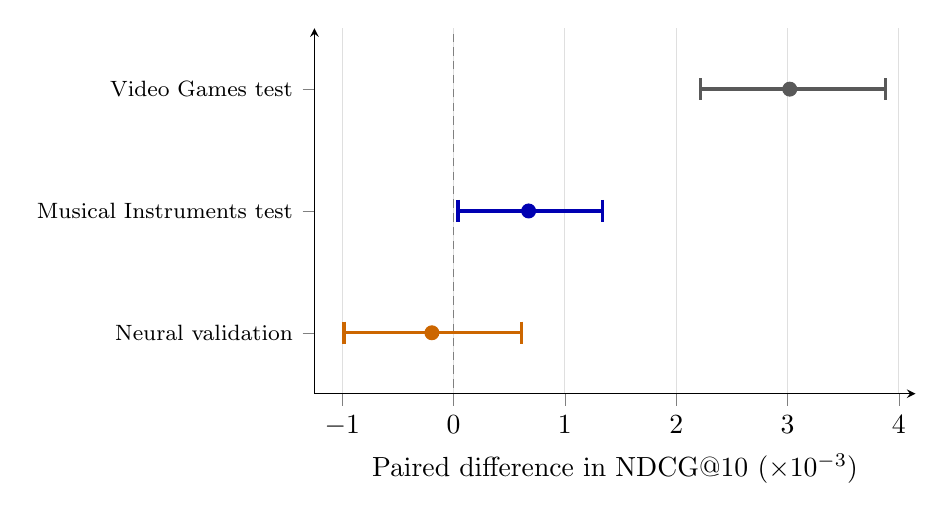
\begin{tikzpicture}
\begin{axis}[
    width=0.76\linewidth, height=2.45in,
    xmin=-1.25, xmax=4.15, ymin=0.5, ymax=3.5,
    xtick={-1,0,1,2,3,4}, ytick={1,2,3},
    yticklabels={Neural validation,Musical Instruments test,Video Games test},
    yticklabel style={font=\footnotesize},
    xlabel={Paired difference in NDCG@10 ($\times 10^{-3}$)},
    xmajorgrids, grid style={gray!25},
    axis x line=bottom, axis y line=left,
    tick align=outside,
]
\addplot[gray,densely dashed,forget plot] coordinates {(0,0.55) (0,3.45)};
\addplot[gray!70!black,very thick,mark=|,mark size=4pt,forget plot] coordinates {(2.216,3) (3.881,3)};
\addplot[gray!70!black,only marks,mark=*,mark size=2.5pt,forget plot] coordinates {(3.020,3)};
\addplot[blue!70!black,very thick,mark=|,mark size=4pt,forget plot] coordinates {(0.040,2) (1.338,2)};
\addplot[blue!70!black,only marks,mark=*,mark size=2.5pt,forget plot] coordinates {(0.674,2)};
\addplot[orange!80!black,very thick,mark=|,mark size=4pt,forget plot] coordinates {(-0.985,1) (0.611,1)};
\addplot[orange!80!black,only marks,mark=*,mark size=2.5pt,forget plot] coordinates {(-0.195,1)};
\end{axis}
\end{tikzpicture}
\caption{Paired NDCG@10 differences with user-cluster bootstrap 95\% intervals. The two test rows compare hybrid with popularity; Musical Instruments is the fixed-method check and Video Games is exploratory. The later neural validation row compares the blended neural challenger with the active hybrid on Musical Instruments, not another test confirmation. Intervals condition on fitted models and one temporal period.}
\label{fig:paired-differences}
\end{figure}

Catalog coverage puts these small absolute scores in context. In Musical Instruments, 12,305 eligible test targets were absent from the 22,753-item training catalog; in Video Games, 22,051 of 35,562 targets were absent. Figure~\ref{fig:catalog-coverage} separates recoverable from absent targets. No reordering of train-known products can recover the latter, so the measured hybrid gain operates within a substantial coverage limit. Nor can recovery of a later review establish that the user would engage with a recommendation.

\begin{figure}[ht]
\centering
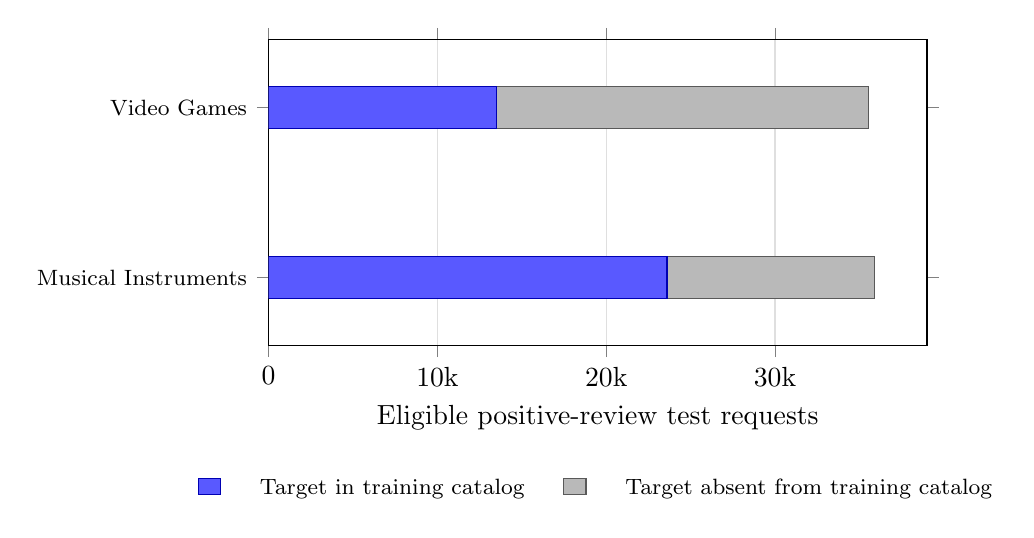
\begin{tikzpicture}
\begin{axis}[
    xbar stacked, width=0.82\linewidth, height=2.15in,
    xmin=0, xmax=39000, bar width=15pt,
    ytick={1,2}, yticklabels={Musical Instruments,Video Games},
    yticklabel style={font=\footnotesize},
    xlabel={Eligible positive-review test requests},
    xtick={0,10000,20000,30000}, xticklabels={0,10k,20k,30k},
    scaled x ticks=false,
    xmajorgrids, grid style={gray!25},
    enlarge y limits=0.4,
    legend style={at={(0.5,-0.4)},anchor=north,legend columns=2,column sep=12pt,draw=none,font=\footnotesize},
    tick align=outside,
]
\addplot[fill=blue!65,draw=blue!70!black] coordinates {(23600,1) (13511,2)};
\addlegendentry{Target in training catalog}
\addplot[fill=gray!55,draw=gray!70!black] coordinates {(12305,1) (22051,2)};
\addlegendentry{Target absent from training catalog}
\end{axis}
\end{tikzpicture}
\caption{Frozen-catalog coverage of eligible test requests. The two segments sum to 35,905 Musical Instruments and 35,562 Video Games requests. Targets absent from the training catalog remain evaluation misses for every model; the chart does not imply those items were available to recommend at request time.}
\label{fig:catalog-coverage}
\end{figure}

\subsection{Neural challenger}
The co-review result raises a more demanding comparison than neural retrieval against popularity alone: can a learned model improve the route already in use? We trained a two-tower retriever on 313,522 chronological pairs from positive Musical Instruments training reviews. Its query tower pools embeddings of up to 20 prior distinct positive items and applies a small residual multilayer perceptron; the item tower embeds training products. Both output normalized 64-dimensional vectors. Training runs for three epochs with in-batch softmax at temperature 0.15, masking duplicate targets and products already known positive for a query so they are not treated as negatives. The model scores the train-known item array exactly; items without positive training support are ineligible for its route, and requests without a supported history fall back to popularity.

The unblended neural model scored 0.001411 NDCG@10 on validation. Blending 40\% neural score with 60\% recent popularity raised it to 0.011774, above recent popularity's 0.010715 but below the active hybrid's 0.011969. Its paired difference from the hybrid was $-0.000195$ [$-0.000985$, 0.000611]; the gate therefore stayed closed. On the already studied test period, the blend scored 0.008357 against 0.008681 for the hybrid. We designed this model after seeing that period's result, so the test comparison is exploratory rather than another fresh confirmation.

\subsection{Evidence the frozen route discards}
The scorer treats up to twenty distinct reviewed items as attraction signals, irrespective of rating or review time. We first checked whether the omitted fields and older items were actually available. The record audit (\texttt{tools/signal\_audit.py}) found 47,459 Musical Instruments validation history slots with a train-recorded rating below four, including 35,444 inside the scorer's window. Another 96,984 slots had no training-row rating for that user--item pair, although only 20,310 referred to products absent from the training catalog. Among distinct history items, 23\% lay beyond the twenty-item window. For all 14,175 validation users with a prior training record, the attached history reproduced that record exactly. The window is thus a scorer choice, not an archive limit.

To isolate each source of evidence, the shadow arms hold the co-review neighbors, candidate set, popularity control, and $\alpha=0.75$ fixed. C1 uses observed dislikes: it subtracts $\gamma$ times the neighbor score of history items rated at most three in training, with $\gamma\in\{0,0.25,0.5,1\}$. C2 instead sets $\gamma=0$ and grades train-recorded four- and five-star items by 0.6 and 1.0, optionally decaying them by $2^{-d/\tau}$ for age $d$ in days and half-life $\tau\in\{90,365,1095\}$; an item with no train rating retains unit attraction. C3 tests a first-positive-review prior for requests without usable co-review neighbors. C4 selects $\alpha$ separately for five history-length buckets. C5 asks about a fixed prefix of the 200 most often positively reviewed training products, excluding the current target and supplied-history items, and uses the archive rating as a hindsight answer. C6 borrows Video Games training activity through users shared with Musical Instruments, firing only when local neighbors are unavailable.

Table~\ref{tab:shadow} scores these arms on 33,993 eligible Musical Instruments validation requests from 13,908 users against the active co-review hybrid at $\alpha=0.75$. Configuration search and interval estimation use the same records. The intervals describe this cohort and do not provide an independent activation test.

\begin{table}[ht]
\centering
\caption{Shadow-profile arms on the Musical Instruments validation cohort, against the active hybrid at 0.011969 NDCG@10. These are exploratory validation results, not fresh confirmations. Intervals are paired user-cluster bootstrap estimates that do not account for selecting each configuration on the same cohort. C1 uses low ratings for repulsion; C2 instead grades and ages observed four- and five-star reviews. Their combination was not tested.}
\label{tab:shadow}
\small
\begin{tabular}{@{}lrrr@{}}
\toprule
Arm & NDCG@10 & $\Delta$ vs active & 95\% interval \\
\midrule
C1 repulsion from sub-four ratings ($\gamma=1$) & 0.012418 & $+0.000449$ & $[0.000266, 0.000626]$ \\
C2 star grading, 1095-day decay & 0.012435 & $+0.000466$ & $[0.000165, 0.000750]$ \\
C3 analogous first-positive-review prior & 0.011824 & $-0.000145$ & $[-0.000270, -0.000028]$ \\
C4 blend weight by history length & 0.012523 & $+0.000554$ & $[0.000062, 0.001057]$ \\
C5 oracle interview (100 prompts, $\gamma=1$) & 0.012840 & $+0.000871$ & $[0.000537, 0.001172]$ \\
C6 adjacent surface, reachable probe & 0.011960 & $-0.000009$ & $[-0.000028, 0.000000]$ \\
\bottomrule
\end{tabular}
\end{table}

C1 changes only the contribution of a history item rated below four: that item now supplies repulsion as well as attraction. At $\gamma=0$, the arm reproduces the active route's 0.011969 on real records, providing a parity check beyond the unit tests. C2's ablation attributes most of its gain to review age rather than star grading. A three-year half-life with flat rating weights moves NDCG@10 from 0.011969 to 0.012381; adding grading contributes another 0.000054. C4 exposes a different pattern. Accuracy peaks for users with one or two recorded items (0.014825) and falls to 0.006784 for those with twenty or more. Where C4 changes the frozen route, it \emph{reduces} the personalized weight from 0.75 to 0.5. On this cohort the fixed blend appears to over-weight long histories, but the bucket weights require independent evaluation.

C5 estimates what asking could add only through a hindsight oracle. For each prompted product, it reads that user's rating across train, validation, and test while withholding the current target; a missing rating supplies no answer. One hundred prompts per request yield about 0.227 recorded answers, or one per 440 prompts. This is coverage of the archive, not a human response rate. C5's $+0.000871$ difference from the active route includes the $+0.000449$ that C1 obtains from already-held low ratings. The difference over C1 is $+0.000422$, but the design cannot isolate newly elicited dislikes because the same repulsion switch also activates existing ones. Even the likes-only 100-prompt cell's $+0.000461$ depends on the hindsight oracle.

The two sparse-history alternatives show different limits. C3 fires on 1,618 requests with no catalog-known history item. Its $-0.000145$ overall difference rescales to about $-0.00305$ on that slice: a prior based on training users' first positive reviews ranks the eventual target worse than the current popularity route, consistent in direction with the MovieLens low-activity result of Ji et al.~\cite{ji2020popularity}. C6 had too little overlap to support a comparison. Only 2,802 training users, roughly one in twenty, appeared in both category archives, and a donor record was reachable for 47 of 33,993 requests (0.14\%). This falls below the design's 5\% reach floor for reading the arm as a comparison.

\subsection{Answering a sentence}
The behavioral route cannot answer a person who states what they want: it reads products in a history, not a sentence. We therefore add a phrase-to-products route that matches a typed sentence against product text and returns its answer beside the unchanged behavioral ranking. Product text is absent from the \texttt{timestamp\_w\_his} files, so we fetch it separately for training-catalog items. Musical Instruments has descriptions for all 22,753 products, titles for 22,751, recorded prices for 14,927, and earlier reviews from 55,981 people. The corresponding Video Games counts are 22,976 products, 22,975 titles, 14,919 prices, and 92,807 earlier reviewers.

An external query-to-product set supplies 1,966 in-catalog Musical Instruments pairs and 3,951 Video Games pairs. Most come from the full official ESCI Shopping Queries Dataset: 1,913 and 3,886 pairs, respectively, after restricting to the US locale and products judged an exact match or acceptable substitute~\cite{reddy2022esci}. Substitute-labeled pairs are included because production retrieval work uses them as coarse training supervision~\cite{kothari2026semantic}. The remaining 53 and 65 pairs come from Amazon-C4, where queries were rewritten from target-product reviews rather than observed in search sessions~\cite{hou2026bridging}. This distinction matters when interpreting the paired diagnostic below.

The lexical matcher uses a standard-library BM25 implementation with postings ordered by item ID ($k_1=1.2$, $b=0.75$). An optional dense route scores the same documents with the 384-dimensional all-MiniLM-L6-v2 sentence encoder. We measure lexical retrieval in both categories and dense retrieval in Musical Instruments, where the embedding artifact exists. The phrase parser scopes negation from one cue to the next, allowing a request to rule out a product class. For the served route, a stated figure acts as a price limit: products priced above it are excluded, while those without a recorded price remain eligible.

We score six wording conditions against the route selected on validation under the same paired gate. Two reconstruct a phrase from a person's earlier reviews, once raw and once scrubbed to product words that appear in fewer than 1\% of listings, limiting the chance that shared product vocabulary alone carries the answer. A third uses another reviewer of the same product as a generalization control. The remaining conditions use the target's exact title, a randomly drawn product title, or an external query pair linked to the eventual target. ESCI queries were observed in shopping search but not from these reviewers at these request times; C4 queries are review-derived rewrites. The exact title and external pair are target-conditioned diagnostics, while the random title is a control. None tests a live request's phrasing. Table~\ref{tab:reach} reports how often each condition retrieves the target and how often the target even enters the shortlist that the confined arm may promote.

\begin{table}[ht]
\centering
\caption{Wording reach on the full test splits (35,905 Musical Instruments requests and 35,562 Video Games requests). Each condition cell gives the number of requests whose answer list contained the eventual target out of the requests where the condition had wording to read, with the fraction in parentheses; the answer list is read without the confinement that produces the measured number, so reach is a diagnostic, not a score. The last row is not a wording condition: it is the share of requests whose target sat inside the top-200 shortlist a confined phrase was allowed to promote at all.}
\label{tab:reach}
\small
\begin{tabular}{@{}lcc@{}}
\toprule
Wording condition & Musical Instruments & Video Games \\
\midrule
Own earlier reviews & 627 / 25,926 (2.42\%) & 390 / 22,320 (1.75\%) \\
Own reviews, scrubbed to rare product words & 584 / 25,926 (2.25\%) & 366 / 22,320 (1.64\%) \\
Another reviewer of the same product & 193 / 25,926 (0.74\%) & 124 / 22,320 (0.56\%) \\
Target product title & 23,596 / 23,600 (99.98\%) & 13,507 / 13,511 (99.97\%) \\
Randomly drawn product title & 263 / 35,905 (0.73\%) & 150 / 35,560 (0.42\%) \\
External pairs (ESCI + C4) & 1,221 / 1,983 (61.57\%) & 1,140 / 2,115 (53.90\%) \\
\midrule
Target inside the promotable shortlist & 11,925 / 35,905 (33.21\%) & 8,267 / 35,562 (23.25\%) \\
\bottomrule
\end{tabular}
\end{table}

The confined wording arm does not clear the gate. With weight 0.25, repulsion 0, and price penalty 0.5, it loses 0.001678 NDCG@10 against the frozen base on the full Musical Instruments test split (95\% interval $[-0.002318, -0.000980]$). It also loses 0.002858 on the exploratory Video Games split (95\% interval $[-0.003598, -0.002195]$). The loss is smaller on the validation cohort used to select the configuration ($-0.001057$, interval $[-0.002147, -0.000042]$), but the arm activates in neither category. Re-scoring the same shortlist with all-MiniLM-L6-v2 is directionally positive on validation ($+0.001048$, interval $[-0.000062, +0.002109]$) without opening the gate. That direction reverses on the full Musical Instruments test split: the encoded version loses 0.001282 (95\% interval $[-0.001944, -0.000577]$).

Only the mixed external-pair condition yields a positive full-split difference among the phrase-like conditions. On Musical Instruments it adds $+0.004931$ with lexical retrieval and $+0.004232$ with encoded retrieval (intervals $[0.004261, 0.005611]$ and $[0.003578, 0.004884]$). Both averages cover all 35,905 test requests, although a pair attaches to only 1,983 of them. On Video Games the lexical difference is $+0.006167$ over all 35,562 requests, with 2,115 attached pairs. These pairs are selected using the known target; they are not queries observed from those reviewers at request time.

A source audit of the fixed lexical run separates the mixed effect. On Musical Instruments, the full ESCI set contributes $+0.002500$ on 1,512 linked requests and C4 rewrites contribute $+0.002431$ on 471. On Video Games, the corresponding contributions are $+0.003883$ on 1,568 and $+0.002284$ on 547. Within ESCI, exact-match pairs contribute $+0.002107$ and $+0.003537$ in the two categories; acceptable substitutes contribute $+0.000393$ and $+0.000346$ and almost never worsen their attached requests. Counting a reached substitute as a hit raises mixed-set reach from 61.57\% to 65.25\% on Musical Instruments and from 53.90\% to 58.49\% on Video Games. Both sources contribute positively at full scale, with a larger per-request effect for the review-derived rewrites. These are descriptive source contributions, and repeated requests share target-linked pairs. The positive interval therefore cannot establish a benefit from observed user queries. Figure~\ref{fig:wording-arm} shows the three regressions for the own-words arm.

Table~\ref{tab:reach} helps locate the failure without multiplying incompatible rates. The target appears in the promotable shortlist for 33.21\% of Musical Instruments requests; unconstrained lexical search over earlier review prose retrieves it for 2.42\% of requests with usable wording. These are marginal rates with different denominators, so their product is not an observed joint ceiling. An exact target title retrieves its product 99.98\% of the time, showing that the index handles target-informed wording, and the mixed external pairs reach the target in 61.57\% of their matched sample. Both the review-prose proxy and shortlist coverage constrain the measured arm. The title probe does not establish retrieval quality for natural queries. Accordingly, the served phrase route reaches the full catalog and leaves behavioral ranking available when the sentence is empty, whereas the measured arm confines phrase promotion and reports its loss.

\begin{figure}[ht]
\centering
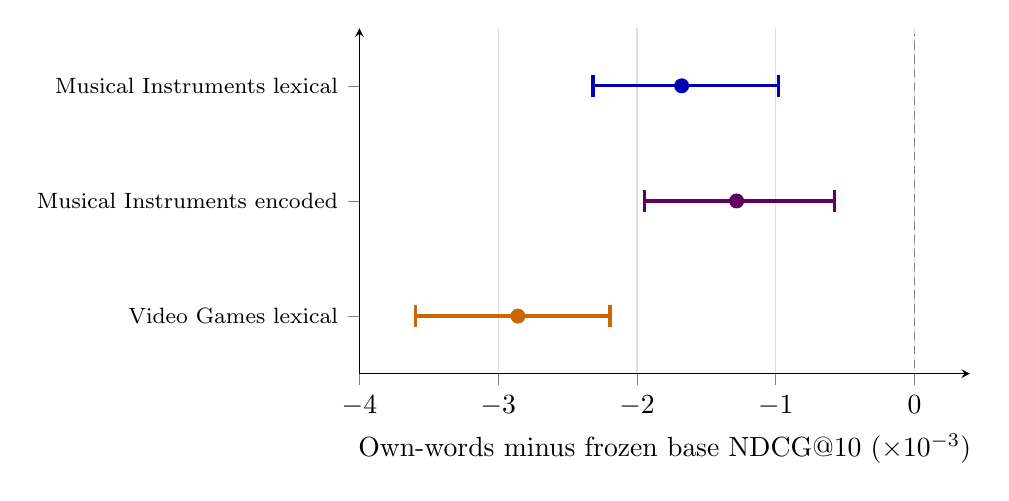
\begin{tikzpicture}
\begin{axis}[
    width=0.77\linewidth, height=2.35in,
    xmin=-4.0, xmax=0.4, ymin=0.5, ymax=3.5,
    xtick={-4,-3,-2,-1,0}, ytick={1,2,3},
    yticklabels={Video Games lexical,Musical Instruments encoded,Musical Instruments lexical},
    yticklabel style={font=\footnotesize},
    xlabel={Own-words minus frozen base NDCG@10 ($\times 10^{-3}$)},
    xmajorgrids, grid style={gray!25},
    axis x line=bottom, axis y line=left,
    tick align=outside,
]
\addplot[gray,densely dashed,forget plot] coordinates {(0,0.55) (0,3.45)};
\addplot[blue!70!black,very thick,mark=|,mark size=4pt,forget plot] coordinates {(-2.318,3) (-0.980,3)};
\addplot[blue!70!black,only marks,mark=*,mark size=2.5pt,forget plot] coordinates {(-1.678,3)};
\addplot[violet!75!black,very thick,mark=|,mark size=4pt,forget plot] coordinates {(-1.944,2) (-0.577,2)};
\addplot[violet!75!black,only marks,mark=*,mark size=2.5pt,forget plot] coordinates {(-1.282,2)};
\addplot[orange!80!black,very thick,mark=|,mark size=4pt,forget plot] coordinates {(-3.598,1) (-2.195,1)};
\addplot[orange!80!black,only marks,mark=*,mark size=2.5pt,forget plot] coordinates {(-2.858,1)};
\end{axis}
\end{tikzpicture}
\caption{Exploratory own-words wording arm against the frozen behavioral base on the full test splits. Points are paired NDCG@10 differences; lines are user-cluster bootstrap 95\% intervals. Lexical retrieval was measured in both categories; encoded retrieval was measured only in Musical Instruments. Both test periods had already been opened by earlier work, so these intervals describe regressions on those cohorts rather than independent confirmation.}
\label{fig:wording-arm}
\end{figure}

The phrase route also has measurable serving cost. Loading 22,753 descriptions and building the lexical index takes 3.1 to 3.2 s at startup. Across 200 scored Musical Instruments requests, lexical answers take 23.1 ms at the median and 30.3 ms at the 95th percentile in process; the corresponding Video Games timings are 22.1 and 36.2 ms. The dense route answers the same 200 Musical Instruments requests in 27.6 and 42.3 ms, after encoding the catalog in 37.4 s on one consumer GPU when its optional dependency is installed. The service retains up to eight earlier sentences in memory so it can answer again using something the person already said.

\section{Guarded Service and Reproducibility}
The service makes the evaluation decision inspectable at request time. Its loopback HTTP API returns baseline, co-review shadow, optional neural shadow, active ranking, and an explicit fallback reason. A saved validation decision selects the active route; empty or unsupported histories and challenger failures return popularity. Before serving, the local model bundle checks its source hash, as do optional neural weights and their training source. A separate phrase route returns its answer beside the behavioral ranking and reports the terms it sought, terms it ruled out, and any stated price limit. This lets a reader distinguish a response to wording from a response to history. Up to eight prior sentences remain only in process memory and disappear when the process stops; submitted histories are not written to disk. A synthetic browser walkthrough uses invented users and products to illustrate these decisions, without changing the measured results.

In-process Python ranking p95 was 0.611 ms for the Video Games replay and 0.760 ms for Musical Instruments. These timings include baseline and co-review challenger scoring but exclude HTTP, loading, concurrency, and network time. Neural batch-ranking has a different measurement scope and is not a direct service-latency comparison. Source, evaluation methods, aggregate JSON results, and tests are available at \url{https://github.com/ahnafnafee/recommendation-decision-lab}. Downloaded reviews, row-level predictions, and fitted weights are not redistributed; the dataset remains available from its owner under its terms~\cite{amazon5core}.

\section{Limitations and Future Work}
The benchmark's 5-core construction retrospectively selects users and products using support across the full corpus. A review is neither an impression nor a purchase nor an unbiased preference label. Our user-cluster intervals hold the fitted models and period fixed; they do not capture shared-item dependence, model refitting, selection across methods, or future conditions. The second category changes the product domain but remains on the same platform. The neural route was designed after that category's test result was known, and one compact architecture cannot represent all learned retrieval methods. A new period or platform would test whether the guarded decision persists.

The profile arms use validation data only, since earlier work had already opened both test periods. Their configurations and intervals come from the same cohort. The positive intervals are therefore descriptive and cannot justify activating a new route; an untouched cohort is needed. We also did not combine the arms, so their interactions remain unknown. The wording arm has a different measurement gap: earlier reviews about other products are not statements of current intent. Removing rare title words barely changes reach, but does not identify why the proxy fails. The external pairs attach through the known target, and the exact-title probe is target-informed. Neither can establish the effect of a live query from these users. Finally, product text must be fetched by a reproducing researcher, and the encoded route was measured only in Musical Instruments, where an embedding artifact was available.

\section{Summary}
The fixed co-review hybrid earned a small improvement over a validation-selected popularity baseline on Musical Instruments. A later neural blend improved on popularity but not on the active hybrid, so the gate stayed closed. Reusing the same decision rule exposed a more actionable distinction: ratings and review times already in the archive produced positive, validation-only shadow differences, whereas simulated questions required about 440 prompts per recorded answer, and prior-review wording could not improve the frozen ranking on either full test split. The phrase route still adds the ability to respond to a stated request, with its answer and evidence shown separately. These outcomes support a restrained deployment principle: compare a challenger with the route actually in use, measure against the catalog it can retrieve, and preserve a clear fallback when the added model or signal has not earned the route.

\begin{thebibliography}{27}
\bibitem{amazon5core} McAuley Lab. \emph{Amazon Reviews'23: Pure IDs (5-Core)}. \url{https://amazon-reviews-2023.github.io/data_processing/5core.html}.
\bibitem{hou2026bridging} Y. Hou, J. Li, X. Fu, Z. He, A. Yan, X. Chen, and J. McAuley. Bridging Language and Items for Retrieval and Recommendation: Benchmarking LLMs as Semantic Encoders. \emph{arXiv:2403.03952}, version 2, 2026. \url{https://arxiv.org/abs/2403.03952}.
\bibitem{ji2023leakage} Y. Ji, A. Sun, J. Zhang, and C. Li. A Critical Study on Data Leakage in Recommender System Offline Evaluation. \emph{ACM Transactions on Information Systems}, 41(3), Article 75, 2023. \url{https://doi.org/10.1145/3569930}.
\bibitem{gusak2025time} D. Gusak, A. Volodkevich, A. Klenitskiy, A. Vasilev, and E. Frolov. Time to Split: Exploring Data Splitting Strategies for Offline Evaluation of Sequential Recommenders. In \emph{Proceedings of RecSys '25}, pp. 874--883, 2025. \url{https://doi.org/10.1145/3705328.3748164}.
\bibitem{covington2016youtube} P. Covington, J. Adams, and E. Sargin. Deep Neural Networks for YouTube Recommendations. In \emph{Proceedings of RecSys '16}, pp. 191--198, 2016. \url{https://doi.org/10.1145/2959100.2959190}.
\bibitem{wang2021crossbatch} J. Wang, J. Zhu, and X. He. Cross-Batch Negative Sampling for Training Two-Tower Recommenders. In \emph{Proceedings of SIGIR '21}, pp. 1632--1636, 2021. \url{https://doi.org/10.1145/3404835.3463032}.
\bibitem{rashid2008preferences} A. M. Rashid, G. Karypis, and J. Riedl. Learning preferences of new users in recommender systems: an information theoretic approach. \emph{SIGKDD Explorations}, 10(2), pp. 90--100, 2008. \url{https://doi.org/10.1145/1540276.1540302}.
\bibitem{crankshaw2016clipper} D. Crankshaw, X. Wang, G. Zhou, M. J. Franklin, J. E. Gonzalez, and I. Stoica. Clipper: A Low-Latency Online Prediction Serving System. \emph{arXiv:1612.03079}, 2016 (later \emph{MLSys '18}). \url{https://arxiv.org/abs/1612.03079}.
\bibitem{hendrickx2021reject} K. Hendrickx, L. Perini, D. Van der Plas, W. Meert, and J. Davis. Machine Learning with a Reject Option: A survey. \emph{Machine Learning}, 113(5), pp. 3073--3110, 2024. \url{https://doi.org/10.1007/s10994-024-06534-x}.
\bibitem{hemmer2023defer} P. Hemmer, L. Thede, M. V\"ossing, J. Jakubik, and N. K\"uhl. Learning to Defer with Limited Expert Predictions. In \emph{Proceedings of AAAI-23}, 37(5), pp. 6002--6011, 2023. \url{https://doi.org/10.1609/aaai.v37i5.25742}.
\bibitem{krauth2020offline} K. Krauth, S. Dean, A. Zhao, W. Guo, M. Curmei, B. Recht, and M. I. Jordan. Do Offline Metrics Predict Online Performance in Recommender Systems? \emph{arXiv:2011.07931}, 2020. \url{https://arxiv.org/abs/2011.07931}.
\bibitem{gilotte2018offline} A. Gilotte, C. Calauz\`enes, T. Nedelec, A. Abraham, and S. Doll\'e. Offline A/B testing for Recommender Systems. In \emph{Proceedings of KDD '18}, 2018. \url{https://arxiv.org/abs/1801.07030}.
\bibitem{hsu2024minimizing} C.-W. Hsu, M. Mladenov, O. Meshi, J. Pine, H. Pham, S. Li, X. Liang, A. Polishko, L. Yang, B. Scheetz, and C. Boutilier. Minimizing Live Experiments in Recommender Systems: User Simulation to Evaluate Preference Elicitation Policies. \emph{arXiv:2409.17436}, 2024. \url{https://arxiv.org/abs/2409.17436}.
\bibitem{gupta2024selection} S. Gupta, H. Oosterhuis, and M. de Rijke. A First Look at Selection Bias in Preference Elicitation for Recommendation. In \emph{CONSEQUENCES'23 workshop at RecSys '23}, 2023. \url{https://arxiv.org/abs/2405.00554}.
\bibitem{huang2020ebr} J. Huang, A. Sharma, S. Sun, L. Xia, D. Zhang, P. Pronin, J. Padmanabhan, G. Ottaviano, and L. Yang. Embedding-based Retrieval in Facebook Search. In \emph{Proceedings of KDD '20}, 2020. \url{https://arxiv.org/abs/2006.11632}.
\bibitem{reddy2022esci} C. K. Reddy, L. M\`arquez, F. Valero, N. Rao, H. Zaragoza, S. Bandyopadhyay, A. Biswas, A. Xing, and K. Subbian. Shopping Queries Dataset: A Large-Scale ESCI Benchmark for Improving Product Search. \emph{arXiv:2206.06588}, 2022. \url{https://arxiv.org/abs/2206.06588}.
\bibitem{kothari2026semantic} N. Kothari, S. Samdani, R. Mallick, P. Gupta, A. Vijay, and S. Kumar. Semantic Retrieval for Product Search in E-Commerce. \emph{arXiv:2606.01504}, 2026. \url{https://arxiv.org/abs/2606.01504}.
\bibitem{reimers2019sbert} N. Reimers and I. Gurevych. Sentence-BERT: Sentence Embeddings using Siamese BERT-Networks. In \emph{Proceedings of EMNLP 2019}, 2019. \url{https://arxiv.org/abs/1908.10084}.
\bibitem{rahmani2024synthetic} H. A. Rahmani, N. Craswell, E. Yilmaz, B. Mitra, and D. Campos. Synthetic Test Collections for Retrieval Evaluation. In \emph{Proceedings of SIGIR 2024}, 2024. \url{https://arxiv.org/abs/2405.07767}.
\bibitem{rahmani2025bias} H. A. Rahmani, V. Ramineni, E. Yilmaz, N. Craswell, and B. Mitra. Towards Understanding Bias in Synthetic Data for Evaluation. In \emph{Proceedings of CIKM 2025}, 2025. \url{https://arxiv.org/abs/2506.10301}.
\bibitem{hussain2026coverage} Z. Hussain and K. Nielbo. The Coverage Illusion: From Pre-retrieval Routing Failure to Post-retrieval Cascades in a Production RAG System. \emph{arXiv:2605.27220}, 2026. \url{https://arxiv.org/abs/2605.27220}.
\bibitem{meng2020splitting} Z. Meng, R. McCreadie, C. Macdonald, and I. Ounis. Exploring Data Splitting Strategies for the Evaluation of Recommendation Models. \emph{arXiv:2007.13237}, 2020. \url{https://arxiv.org/abs/2007.13237}.
\bibitem{hidasi2023flaws} B. Hidasi and {\'A}. T. Czapp. Widespread Flaws in Offline Evaluation of Recommender Systems. In \emph{Proceedings of the 17th ACM Conference on Recommender Systems}, 2023. \url{https://arxiv.org/abs/2307.14951}.
\bibitem{schnabel2022here} T. Schnabel. Where Do We Go From Here? Guidelines For Offline Recommender Evaluation. \emph{arXiv:2211.01261}, 2022. \url{https://arxiv.org/abs/2211.01261}.
\bibitem{pan2023sine}
Yunzhu Pan, Chen Gao, Jianxin Chang, Yanan Niu, Yang Song, Kun Gai, Depeng Jin, and
Yong Li.
\newblock Understanding and Modeling Passive-Negative Feedback for Short-video
  Sequential Recommendation.
\newblock In {\em Proceedings of the 17th ACM Conference on Recommender Systems}, 2023.
\newblock arXiv:2308.04086. \url{https://arxiv.org/abs/2308.04086}.

\bibitem{wang2023negative}
Yueqi Wang, Yoni Halpern, Shuo Chang, Jingchen Feng, Elaine Ya Le, Longfei Li, Xujian
Liang, Min-Cheng Huang, Shane Li, Alex Beutel, Yaping Zhang, and Shuchao Bi.
\newblock Learning from Negative User Feedback and Measuring Responsiveness for
  Sequential Recommenders.
\newblock In {\em Proceedings of the 17th ACM Conference on Recommender Systems,
  Industry Track}, 2023.
\newblock arXiv:2308.12256. \url{https://arxiv.org/abs/2308.12256}.

\bibitem{ji2020popularity}
Yitong Ji, Aixin Sun, Jie Zhang, and Chenliang Li.
\newblock A Re-visit of the Popularity Baseline in Recommender Systems.
\newblock In {\em Proceedings of the 43rd International ACM SIGIR Conference on
  Research and Development in Information Retrieval}, 2020.
\newblock arXiv:2005.13829. \url{https://arxiv.org/abs/2005.13829}.

\end{thebibliography}

\end{document}
